\subsection{Objetivo 7 --- níveis intermediários são um limite mais realista?}

\textit{Analisar se níveis intermediários de Oracle podem representar estimativas de
limite superior mais conservadoras e mais próximas do desempenho de métodos reais.}

\textbf{A resposta é não}, e o experimento identifica a razão estrutural.

Defina $N^{*}$ como o menor $N$ tal que $\On{N} <$ votação majoritária --- o nível em
que o Oracle deixa de ser otimista.

\begin{table}[htbp]
\centering
\caption{$N^{*}$ por modo, com $M=100$.}
\begin{tabular}{lrrrr}
\toprule
Modo & Mediana & IQR & Média & Folds com $N^{*}>50$ \\
\midrule
GA            & 52 & $[51, 55]$ & 51.9 & 79.3\% \\
Bagging       & 53 & $[51, 56]$ & 54.4 & 81.4\% \\
Random Forest & 53 & $[51, 56]$ & 53.0 & 79.3\% \\
\bottomrule
\end{tabular}
\end{table}

Friedman $p=0.40$: \textbf{os três modos têm o mesmo $N^{*}$, e ele fica em
$N\approx M/2$}. Não é coincidência empírica. O mecanismo não é a identidade
$\On{M/2+1}\equiv\mvr$ --- essa afirmação, feita em versões anteriores, é falsa ---
mas um \emph{sanduíche}:
\begin{equation}
\On{M/2+1} \;\le\; \mvr \;\le\; \On{M/2}.
\end{equation}

A votação acerta sempre que mais da metade do pool acerta, logo $\mvr\ge\On{51}$;
e ela só pode ganhar, além disso, os empates $50$--$50$, logo nunca passa de
$\On{50}$. O sanduíche foi verificado em \textbf{660 de 660} folds binários, mas a
igualdade $\mvr=\On{51}$ vale em apenas $508$ deles ($77\%$): nos demais $23\%$ os
empates são desfeitos a favor, com excesso médio de $+0.0035$.

A distinção não é um detalhe --- é ela que dá o valor de $N^{*}$. Como $N^{*}$ é o
primeiro nível \emph{estritamente} abaixo do \mvr{}, e $\On{51}=\mvr$ não satisfaz
``$<$'', os empates empurram $N^{*}$ de $51$ para $52$ ou mais, que é exatamente
onde as medianas caem.

\paragraph{O limite é do caso binário.} $22$ das $29$ bases são binárias. Nas $7$
multiclasse a votação é por pluralidade e um classificador correto não precisa de
$51$ votos para vencer, então o sanduíche não vale --- e $N^{*}$ desce de forma
significativa:

\begin{table}[htbp]
\centering
\caption{$N^{*}$ mediano por cardinalidade de classes.}
\begin{tabular}{lrrrr}
\toprule
grupo & bases & GA & Bagging & RF \\
\midrule
binárias    & 22 & 53.4 & 53.7 & 53.5 \\
multiclasse &  7 & 44.4 & 48.1 & 47.3 \\
\bottomrule
\end{tabular}
\end{table}

\noindent
Mediana $53.7$ contra $47.6$, Mann-Whitney $p=2.7\times10^{-6}$. Dentro de cada
grupo os modos continuam empatados ($p=0.71$ e $p=0.37$).

Disso decorre a resposta ao objetivo, \textbf{restrita aos problemas binários}:

\begin{itemize}
\item Para $N \ll M/2$ a curva está \textbf{saturada}: os três modos ficam entre
$0.988$ e $0.998$ em $N=1..5$, e $\On{5}\ge\mvr$ em $100\%$ dos $870$ folds. As
diferenças entre modos são estatisticamente reais ($p<0.001$) mas de magnitude
$0.002$--$0.004$. Mais conservador que \On{1}, sim; perto de um método real, não.

\item Para $N\approx M/2$ a curva \textbf{já é} a votação majoritária, sob outro
nome. Não acrescenta informação.

\item \textbf{Não existe faixa intermediária útil} entre as duas.
\end{itemize}

\begin{figure}[htbp]
\centering
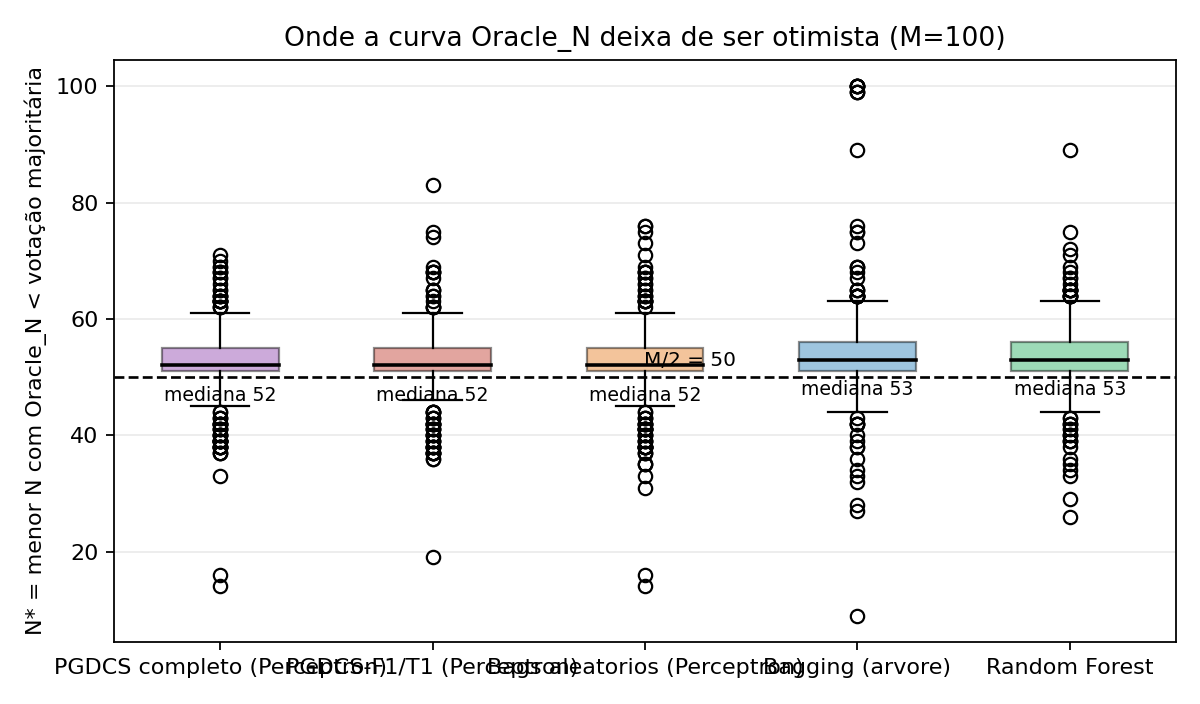
\includegraphics[width=0.72\textwidth]{figuras/fig3_nstar.png}
\caption{Distribuição de $N^{*}$. A concentração em torno de $M/2$ nos três modos é o
que impede qualquer nível intermediário de servir como limite realista.}
\end{figure}

\paragraph{O que substitui a ideia original.} O objetivo 7 buscava uma estimativa
conservadora e alcançável. Ela existe, mas não é ``\On{N} para algum $N$''; é a folga
$\On{1}-\mvr$ ponderada pela fração dela que métodos reais recuperam. Medido: mesmo
tomando o melhor de dez métodos dinâmicos escolhido \emph{a posteriori} no teste, a
recuperação fica em $24.0\%$ (GA), $15.0\%$ (Bagging) e $14.2\%$ (RF), com medianas
bem menores ($0.167$, $0.108$, $0.091$) e recuperação \emph{exatamente zero} no
primeiro quartil de Bagging e RF.

\textbf{Correção.} Versões anteriores apresentavam
\begin{equation}
\mvr + 0.15\,\bigl(\On{1}-\mvr\bigr)
\end{equation}
como ``limite superior operacional''. Não é um limite: $0.15$ é a recuperação
\emph{média} dos pools de árvore, e uma média é ultrapassada por metade da massa.
Medido nos folds de árvore, $37.7\%$ deles recuperam mais que $0.15$. A expressão é
uma \textbf{estimativa}, $\widehat{\mathrm{Acc}}_{DS}$, e deve ser lida como tal.

Quem quiser de fato uma cota precisa de um quantil alto da distribuição de
$R=\text{recuperação}$, não da sua média:
\begin{equation}
\widehat{\mathrm{Acc}}_{DS} = \mvr + \overline{R}\,\bigl(\On{1}-\mvr\bigr),
\qquad
\mathrm{cota}_{95} = \mvr + Q_{0.95}(R)\,\bigl(\On{1}-\mvr\bigr),
\end{equation}
com $Q_{0.95}(R)=0.50$ nos pools de árvore --- mais de três vezes a média. E os dois
números descrevem a mesma distribuição em que $31\%$ dos folds recuperam
\emph{nada} ($R\le 0$). Ambos permanecem otimistas, porque $R$ é medido escolhendo o
melhor método no próprio teste.

\paragraph{Robustez à métrica.} A metodologia do subprojeto pede precisão, revocação,
F1 e acurácia balanceada além da acurácia --- a preocupação legítima sendo que a
acurácia bruta esconda a classe minoritária, num catálogo que chega a IMB $71.5$. As
quatro métricas foram gravadas para \emph{todo} fusor. Em acurácia balanceada tudo
cai, mas de forma quase uniforme, e a folga \emph{cresce}:

\begin{table}[htbp]
\centering
\caption{Acurácia \emph{versus} acurácia balanceada.}
\begin{tabular}{lrrrrrr}
\toprule
Modo & \On{1} & \On{1} balanc. & \mvr & \mvr balanc. & Folga & Folga balanc. \\
\midrule
GA            & 0.9976 & 0.9967 & 0.7784 & 0.7368 & 0.2192 & 0.2599 \\
Bagging       & 0.9951 & 0.9923 & 0.8467 & 0.8163 & 0.1484 & 0.1760 \\
Random Forest & 0.9970 & 0.9949 & 0.8549 & 0.8214 & 0.1421 & 0.1735 \\
\bottomrule
\end{tabular}
\end{table}

O \On{1} é quase insensível ao desbalanceamento --- basta \emph{um} classificador do
pool acertar a instância minoritária --- enquanto o \mvr{} precisa que $51$ acertem,
e é aí que a minoria se perde. Nos \emph{ranks} de fusor a única mudança sistemática
é o DCS puro melhorar $0.3$--$0.4$ posições (OLA vai de \emph{rank} $6.38$ para
$6.00$ no RF), o que faz sentido --- escolher o competente na vizinhança ajuda numa
região minoritária. Mas em nenhum modo isso muda o topo: KNORA-U, META-DES, \mvr{} e
combinação suave continuam empatados na frente, e OLA e LCA continuam no fundo.
\textbf{Nenhuma conclusão deste relatório depende da escolha da métrica.}
